Sequential data and timeseries, causal relations, consequences of actions

Modelling temporal data is of fundamental interest in many branches of science.
This is understandable, since natural organisms inhabit a dynamic environment and
it is natural organisms, such as ourselves, that easily draw our attention and raise questions
deserving a scientific answer. The accuracy of the predictions, based on earlier observations,
is indeed a property that can easily affect the survival of the forecaster.  

Causality and consequences of actions are concepts tied to the passage of time.
Thus it is often time, that dictates the natural ordering of the datapoints
in sequential data. It is however not necessarily so, and any other single
physical dimension may also be used.

Commonly the sequential data is a result of making \emph{measurements} on a
\emph{system} of interest. In order to answer questions quantitatively,
the system and the measurements should be mathematically \emph{modelled}. The class of mathematical
models for dynamical systems we will be concerned with are called \emph{state space models} (SSMs).
Intuitively, SSMs make a clear distinction between the system and the measurements. At any instant,
the system is at a certain \emph{state}. In general, it is this state and its evolution that we are interested in.
However the state is \emph{hidden} (or \emph{latent}) and the inference on the state has to be made entirely
based on the measurements.  Often at least part of the state is conceptually part of the measurements,
but even this part of the state is still latent, since the measurements are always assumed to be \emph{noisy}.
To give a simple but often used example, let us consider the target tracking problem. In this case the state
could include the position, velocity and acceleration of the target and our measurements could consists
of a sequence of noisy angular readings between the line of sight and a reference line. This situation is
known as \emph{bearings-only target tracking} \parencite{ristic2004beyond}.

The noisiness forces us to assume a probabilistic framework. In this thesis the viewpoint
is decidedly \emph{Bayesian}. In Bayesian statistics, ideally, the complete answer
is always the \emph{posterior probability distribution}. Thus instead of answering
with a single value or a value with error bounds, the answer is the probability
density function of the interesting quantity given data. It is important to higlight,
however, that Bayesian statistics can be used to treat many kinds of uncertainty
\parencite{Sarkka2012a}. For example, the instruments used to obtain the measurements often incur
actual physical randomness modeled with Bayesian statistics, whereas the model parameters might in reality have some
exact ``true'' values, but our uncertainty about those values is still quantified with
Bayesian statistics. Thus applying statistical methods to a problem does not imply
that the problem is actually random.

SSMs are a general framework and in any specific situation prior knowledge of the
system has to be brought in. This prior knowledge is not necessarily very specific,
for example in ballistic target tracking it might include the assumption that Newton's
laws are applicable. The mathematical form of the dependence
between the measurements and the state has to be formulated as well as the dependence
of the state on its predecessors. Usually one is able only to specify the 
\emph{parametric} form for these equations. This results in a model with a set
of unknown parameters, denoted with $\Th$. Then, in order
to complete the model, these parameters need to be estimated based on some available
training data. This is sometimes, at least
in control engineering, known as \emph{system identification}. In this thesis,
it is assumed that the parameters are static, i.e. that they stay constant
as time passes. This is then an important distinction between the states and
the parameters, in this thesis.

In general, assuming the aforementioned distinction between parameters and states, there are two separate but
interconnected estimation problems in SSMs: that of the states and that of the parameters. The interest might
lie in either one or both, depending on the model. Traditionally, state
estimation, given measurements up to the current instant, is known as \emph{filtering}.
The term can be thought to relate to the idea of filtering the noise out of the measurements
in order to observe the states. Given all the measurements, including the ones
\emph{after} the current time point, state estimation is called \emph{smoothing}.
Clearly, in order to do smoothing, one has to first collect all the measurements
and then go on with the estimation. Filtering, on the other hand, is an \emph{on-line}
procedure, i.e. the estimates can be updated every time a new measurement arrives.

A distinction is drawn in this thesis between \emph{linear} and \emph{nonlinear}
models. The linear model can be thought of as a special case of a nonlinear model,
so that the linear case would be implicitely covered by only considering nonlinear models.
Linear models are considered separately for the simple reason, that in their case, closed
form solutions exist. The Bayesian solution of the filtering problem for a linear system
with Gaussian noise is given by the celebrated \emph{Kalman filter} \parencite{Kalman1960}.

Our focus in this thesis is in the parameter estimation problem for the nonlinear case.
Depending on the method, this requires either the filtering or filtering and smoothing
solutions of the state estimation problem. For reasons of computational complexity, we will not however try to pursue
the the complete Bayesian solution of finding the posterior distribution. We will settle
for a point estimate called the \emph{maximum a posteriori} (MAP), which is the mode
of the posterior distribution. Under an assumed \emph{uniform} prior distribution,
the MAP estimate becomes equivalent with the \emph{maximum likelihood} (ML) estimate.
As will be seen, the distinction between these two, from the perspective of the
estimation equations, is not fundamental.

The structure of the thesis is as follows. We begin with the background, where
the SSMs are covered in necessary detail, the Bayesian optimal filtering
and smoothing equations are derived and the role of the static parameters is elaborated
on. Following the introduction we focus on on state estimation, first for linear
and then for nonlinear systems. The Kalman filter is introduced here as is the
concept of Gaussian filtering, a deterministic approximation used for nonlinear systems 
in this thesis. The third chapter is considered with the two methods
of parameter estimation we are comparing: the gradient based nonlinear optimization alternative
and the expectation maximization algorithm. The methods are analyzed in sufficient
theoretical detail in order to draw conclusions about the behavior of the methods
in the results section. The results section has three subsection: the analytical 
comparison of the competing algorithms from the point of view of convergence
and complexity, application with simulated data and an application with real world data.

State and measurement and modeling

Markov chain

Parameters, when and why are they interesting?

Bayesian approach, priors, probability distributions, uncertainty

Linear Gaussian 
  


Nonlinear Gaussian
  Bearings-only target tracking
  Stochastic volatility



 

\begin{example}[Endoathmospheric flight of a ballistic object]
\label{ex:ballistic}
Let us consider a situation where a ballistic object is launched
from the ground into the air. We assume that the situation is governed by Newtonian
mechanics and that the object experiences a constant known gravitational
force. In reality, there would also exist a considerable \emph{drag} force
caused by the (possibly moving) air, the magnitude of which is dependent
on the altitude and the velocity of the object \parencite{ristic2004beyond}. 

We wish to apply a linear state space model to the system. We assume
that owing to the unknown wind conditions, the drag force will not be
explicitly modeled. This omission is compensated by introducing
uncertainty into the dynamics with an additive stochastic process.
The only modeled force is then the constant gravitational force.

We obtain a sequence of range measurements with a radar,
so that our data consists of the noisy two dimensional locations 
of the object as measured at time points $\brac{t_k}_{k=1}^T$.
We assume a constant interval $\tau$ between the time points.

Newton's laws are specified in continous time,  where
the dynamics can now be written as
\begin{align}
	\dod{\x(t)}{t} &= \v{F}\x(t) + \gv{\beta}(t)
	\label{eq:ct_linear}
\end{align}
with
\begin{align}
	\x(t) &= \bm{x(t) & \dot{x}(t) & \ddot{x}(t) & y(t) & \dot{y}(t) & \ddot{y}(t)}^\tr\\
	\v{F}&=\bm{
	&&1&&&\\
	&&&1&&\\
	&&&&1&\\
	&&&&&1\\
	&&&&&\\
	&&&&&\\
	}
	\label{tablelabel}
\end{align}

To discretize the dynamics, we will apply a simple integration scheme where 
$\x(t)=\x(t_k)$ when $t\in\brak{t_k,t_{k+1}}$ \parencite{bar2004estimation}.
In this model, the state will constain the two dimensional location and
its first and second time derivatives, i.e the velocity and the acceleration:
\begin{align}
	\x_k &= \bm{x_k & \dot{x}_k & \ddot{x}_k & y_k & \dot{y}_k & \ddot{y}_k }^\tr,
\end{align}
where
\begin{align}
	x_k &= x(t_k)&\dot{x}_k &= \eval{\dod{x(t)}{t}}_{t=t_k}&\ddot{x}_k &= \eval{\dod[2]{x(t)}{t}}_{t=t_k}
\end{align}
and simililarly for $y_k$, $\dot{y}_k$ and $\ddot{y}_k$.
Only the position is observed, so that in the absence of measurement noise we 
would have $\y_k=\bm{\x_k & \y_k}$.
Then
\begin{align*}
	\x_k &= \v{A}\xkk+\v{L}\v{v}_{k-1}&\v{v}_{k-1}\sim \N{\v{0}}{\v{B}}\\
	\yk &=\v{H}\xk+\v{r}_k & \v{r}_{k}\sim \N{\v{0}}{\v{R}},
\end{align*}
where
\begin{align*}
	\v{A}&=\bm{
	1&\tau&\sfrac{\tau^2}{2}&&&\\
	&1&\tau&&&\\
	&&1&&&\\
	&&&1&\tau&\sfrac{\tau^2}{2}\\
	&&&&1&\tau\\
	&&&&&1\\
	}\\
	\v{L} &= \bm{
	\sfrac{\tau^2}{2} & \tau & 1 &  &  &\\
	&&&\sfrac{\tau^2}{2} & \tau & 1
	}^\tr\\
	\v{B} &= \bm{\sigma_x^2 & \\ & \sigma_y^2}
	\v{R} &= \bm{\sigma_r^2 & \\ & \sigma_r^2}
\end{align*}
Simulating the model can be done by starting from an initial
state $\x_0$. We will choose the following initial parameters:
\begin{align}
	x_0 &= \SI{0}{m/s} & \dot{x}_0&=\cos(\alpha_0)v_0 & \ddot{x}_0&=\SI{0}{m/s^2}\\
	y_0 &= \SI{0}{m/s} & \dot{y}_0&=\sin(\alpha_0)v_0 & \ddot{y}_0&=\SI{-9.81}{m/s^2},
\end{align}
where
\begin{align}
	\alpha_0 &= \ang{50} & v_0&=\SI{40}{m/s}.
\end{align}
 The amount of drift in the forces affecting the object can be
 controlled by the standard deviations $\sigma_x$ and $\sigma_y$.
These determine the standard deviations in the horizontal and vertical
components of the force per a single time step of duration $\tau$.
We will set 
\begin{align}
	\sigma_x&=\tau\,\si{m/s^2}\\
	\sigma_y&=\SI{0}{m/s^2}.
\end{align}
 %
 The results of the simulation are presented in Figure~\ref{fig:ballistic}
 
\end{example}

\begin{figure}[htb]%
    \centering%
    \begin{subfigure}[b]{0.5\textwidth}%
    	\centering%
    	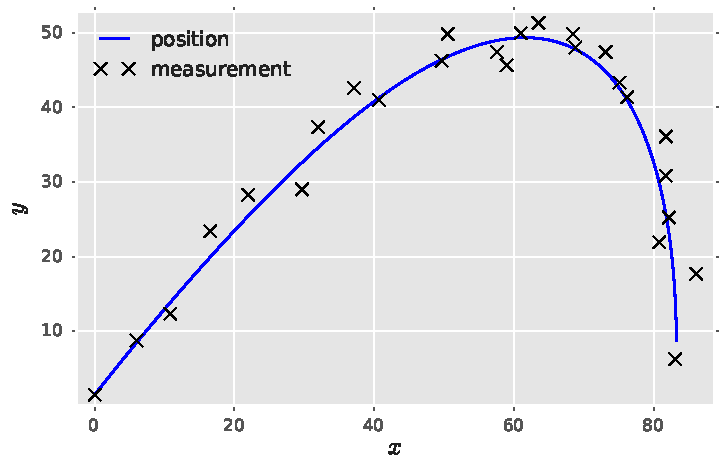
\includegraphics[width=\textwidth]{img/ex1_pos_meas}%
    	\caption{The noisy measurements are plotted with crosses. The initial point is at the origo.}%
		\label{fig:ballistic_flight}%
    \end{subfigure}
    \begin{subfigure}[b]{0.5\textwidth}%
    	%\captionsetup{margin=0pt}
    	\centering%
		\includegraphics[width=\textwidth]{img/ex1_x2}%
    	\caption{$x$ velocity}%
		\label{fig:ballistic_x2}%
    \end{subfigure}%
    \begin{subfigure}[b]{0.5\textwidth}%
    	\centering%
		\includegraphics[width=\textwidth]{img/ex1_x5}%
    	\caption{$y$ velocity}\label{fig:ballistic_x5}%
    \end{subfigure}
	
    \begin{subfigure}[b]{0.5\textwidth}%
    	\centering%
		\includegraphics[width=\textwidth]{img/ex1_x3}%
    	\caption{$x$ acceleration}\label{fig:ballistic_x3}%
    \end{subfigure}%
    \begin{subfigure}[b]{0.5\textwidth}
    	\centering%
		\includegraphics[width=\textwidth]{img/ex1_x6}%
    	\caption{$y$ acceleration}\label{fig:ballistic_x6}%
    \end{subfigure}%
	\caption{A simulation of the the ballistic object in 
	Example~\ref{ex:ballistic}.}
	\label{fig:ballistic}
 \end{figure}
 

